\section{Possible explanations}
\subsection{Causes for the gender gap in the literature}


\subsection{Increased sorting}
\bitem
\item Regressions above do not control for observable characteristics.
\item If women with stronger ability sort themselves:
\bitem
	\item Increasingly in denser cities.
	\item This sorting is stronger than men.
\eitem
\item This would generate faster decrease of the gender gap in denser places.
\eitem


Suppose wages are determine as follows:
\beqns
	y_{igr}=X_{igr}\gamma+\varepsilon_{igr}
\eeqns
taking averages by gender at the CZ level we have:
\beqns
	\bar{y}_{gr}=\bar{X}_{gr}\gamma+\bar{\varepsilon}_{gr}
\eeqns
therefore:
\beqns
\bar{y}_{mr}-\bar{y}_{fr}=(\bar{X}_{mr}-\bar{X}_{fr})\gamma+\bar{\varepsilon}_{mr}-\bar{\varepsilon}_{fr}
\eeqns
so by running the regression:
\beqns
\bar{y}_{mr}-\bar{y}_{fr}=\beta\log(density)_r+\bar{\varepsilon}_{mr}-\bar{\varepsilon}_{fr}
\eeqns
$\beta$ would be reflecting the correlation between CZ population density and the average gap between male and female characteristics. This omitted variable problem is easily resolved by running the regression:
\beqn
\bar{y}_{mr}-\bar{y}_{fr}=(\bar{X}_{mr}-\bar{X}_{fr})\gamma+\beta\log(density)_r+\bar{\varepsilon}_{mr}-\bar{\varepsilon}_{fr}
\eeqn
\paragraph{Things to have in mind}
\bitem
	\item These regressions impose the same return to observable characteristics for men and women in all CZ. Differential returns across CZ will go into the residual.
\eitem 

\paragraph{Procedure}

\subparagraph{Aggregate level data}
I run the regression
\beqns
	\bar{y}_{mr}-\bar{y}_{fr}=\alpha_t +(\bar{X}_{mr}-\bar{X}_{fr})\gamma_t+\beta_t\log(density)_r+u_{rt}
\eeqns
where I allow the return to observable characteristics to vary by year. The main interest is looking at the resulting evolution of $\beta_t$.

\subparagraph{Individual level data}
This just allows for a more flexible variation on the returns of age birth place. Here the estimation is done in two steps:
\benu
	\item Estimate the regression:
	\beqn
		y_{igr}=X_{igr}\gamma+\lambda_{gr}+\varepsilon_{igr}
	\eeqn
	\item Compute CZ-adjusted wage gap:
	\beqns
		\tau_r=\lambda_{mr}-\lambda_{fr}
	\eeqns
	\item Run the regression:
	\beqns
	\tau_r=\alpha_t+\beta_t\log(density)_r
	\eeqns
\eenu

I prefer this method as it exploits the individual level data in a richer way.


\subparagraph{Results} 
 Overall individual level characteristics have limited value in accounting for the cross-sectional gradient and time-variation. Industry-level dummies are much more successful in accounting for the 1970-1990 period.


\FloatBarrier
\begin{figure}[!h]
\centering
\caption{Coefficient on population density $ \beta_t $ controlling for worker characteristics}
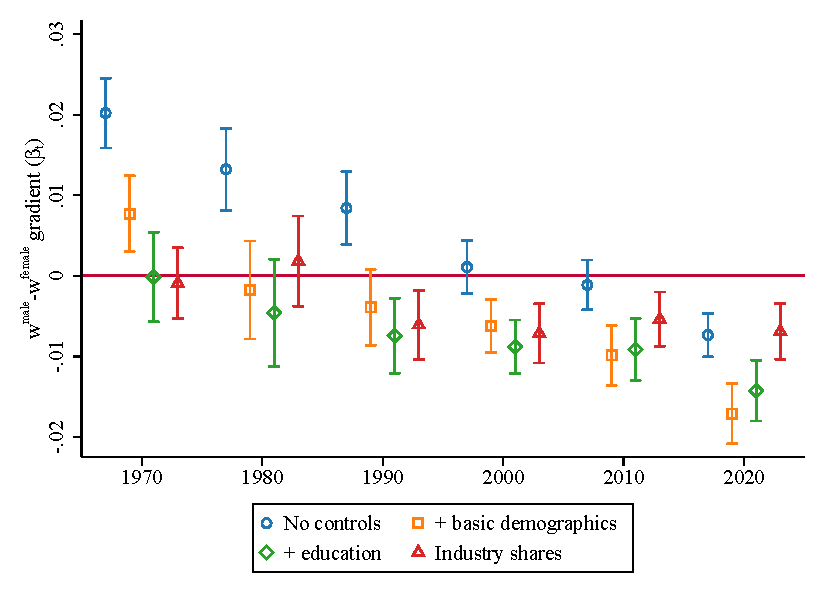
\includegraphics[width=.6\textwidth]{../2_analysis/output/figures/with_control_gradients_l_czone_density_full_time}
\par \begin{minipage}[h]{\textwidth}{\scriptsize\textbf{Note:} figure restricts to CZ with more than 1 people per km$^2$. The regressions are done on data aggregated at the CZ level. Bars show 95\% robust confidence intervals.}\end{minipage}
\end{figure}

\FloatBarrier

\begin{figure}[!h]
\centering
\caption{Coefficient on population density $ \beta_t $ controlling for worker characteristics}
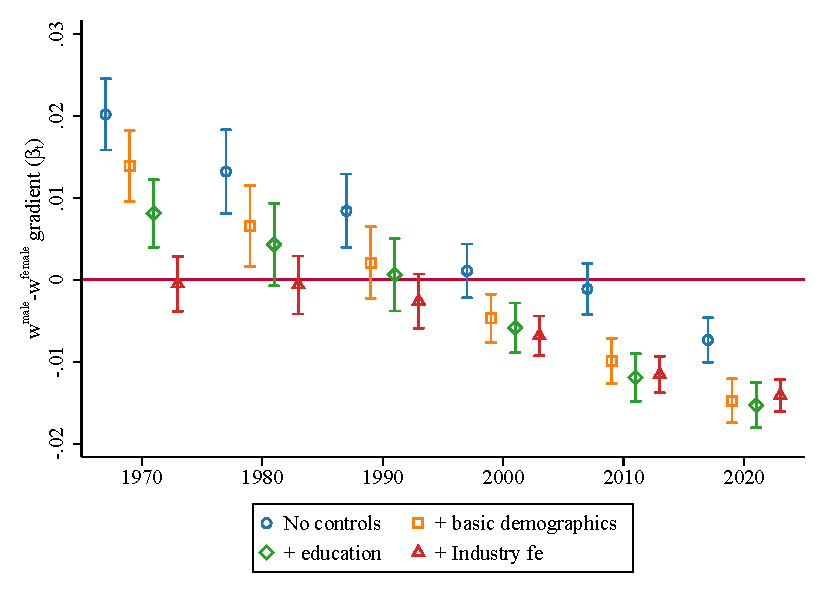
\includegraphics[width=.6\textwidth]{../2_analysis/output/figures/with_control_gradients_individual_l_czone_density_full_time}
\par \begin{minipage}[h]{\textwidth}{\tiny\textbf{Note:} figure restricts to CZ with more than 1 people per km$^2$. The regressions are done on data aggregated at the CZ level after residualizing individual-level characteristics. Bars show 95\% confidence intervals. Errors clustered at the CZ-level.}\end{minipage}
\end{figure}


\subsection{Changes in CZ industrial structure}
Figure 4 suggests that changes in the CZ industrial structure can go a long way in accounting for the cross-sectional variation. Here I do several exercises to explore this possibility.

\subsubsection{Some national level facts}
\paragraph{Women are initially concentrated in low-pay industries}
See \href{https://www.dropbox.com/s/lfpo3q5i9mvq8ry/employment_distribution_gender_full_time.png?dl=0}{here} $=> $ regions specialized on these high-pay industries will show a higher gender gap.


\paragraph{Getting a workable definition of a high-wage 70s industry}
A high wage industry is one that has a high worker-adjusted average pay in 1970. To be more precise, using individual level data in 1970 I run:
\beqn
y_{i}=X_{i}\beta+\lambda_{s}
\eeqn
where $s$ denotes the industry.  I define an industry as having high-pay if they are in the top quartile of the $\lambda_{s}$ distribution. When computing the quartiles, industries are weighted by employment share so that in 1970 each quartile accounts for 25\% of the national level.

\paragraph{High pay industries were disproportionately concentrated in denser places in 1970 \href{https://www.dropbox.com/s/dwse5a96c5xl2xx/high_pay_ind_density_full_time.png?dl=0}{(graph)}}

\paragraph{High pay industries are in decline at the national level \href{https://www.dropbox.com/s/nwr1ozinncqehnh/employment_share_quartile_by_year_full_time.png?dl=0}{(graph)}} decline at the national level starts in 1990


\paragraph{High pay industries belong mainly to manufacturing \href{https://www.dropbox.com/s/kle6o99of1zxtlo/high_pay_industries.txt?dl=0}{(log file)}} the rest are mostly oil or utilities.

\paragraph{Employment share in highly paid industries accounts for most cross-sectional gradient on density during 1970-90 \href{https://www.dropbox.com/s/qgp2oos8g379e36/controlling_high_wage_industries_full_time.png?dl=0}{(graph)}} it also accounts for the time variation from 1970-90s. There's still something going on from 90 to 20

\paragraph{What can be happening:}
\bitem
	\item High wage industries are in decline in denser places... then the decline decline in male advantage comes from employment reallocation.
	\item It can be that at the start of the period, women are getting better access these industries. \textit{I think for the 90's this seems to be the case.}
\eitem



\paragraph{These industries continue to be highly paid industries}
See here






\paragraph{Denser CZ are more specialized in 70s high pay industries}


See \href{https://www.dropbox.com/s/dwse5a96c5xl2xx/high_pay_ind_density_full_time.png?dl=0}{here}

\paragraph{70s high-pay industries decline disproportionately more in denser places}


\paragraph{Women }
\href{https://www.dropbox.com/s/dwse5a96c5xl2xx/high_pay_ind_density_full_time.png?dl=0}{here}



